\chapter{Validación experimental: Conducto Nº5 del reactor RA-6}
% \label{chap:validacion-ra6}

El presente capítulo se validará el método de remuestreo de partículas mediante histogramas multidimensionales desarrollado en este trabajo. Para ello, se lo aplicará al conducto Nº5 del reactor RA-6, un reactor nuclear de investigación tipo pileta ubicado en el Centro Atómico Bariloche (CAB), Argentina.

El RA-6 cuenta con 5 conductos de extracción de neutrones diseñados para transportar haces desde el núcleo hacia diferentes instalaciones experimentales. En particular, el Departamento de Neutrones del CAB ha desarrollado espectrometría basada en la técnica de tiempo de vuelo (TdV) sobre el conducto Nº5. Esto se realiza utilizando un instrumento denominado \textit{chopper}, cuya función es pulsar el haz de neutrones. Midiendo el tiempo que tardan los neutrones en viajar desde el \textit{chopper} hasta un banco de detectores de \textsuperscript{3}He, se obtiene el espectro de energía del haz mediante TdV.

A su vez, el Departamento de Neutrones ha realizado simulaciones Monte Carlo del RA-6 utilizando el código \texttt{OpenMC} con el objetivo de estimar la distribución espectral en el banco de detectores. Sin embargo, debido a la baja probabilidad de que un neutrón simulado desde el núcleo alcance dicha región, una simulación directa resulta computacionalmente inviable.

Para superar esta limitación, se empleó una segmentación geométrica del problema. En una primera simulación desde núcleo, el Departamento de Neutrones registró un archivo de partículas en la entrada del conducto Nº5. Con este archivo de partículas se generó una fuente distribucional con el método de histogramas multidimensionales. Esta fuente se utilizó como entrada en una segunda simulación de \texttt{OpenMC}, que modela exclusivamente el conducto Nº5 hasta el banco de detectores.

Este enfoque permite generar una mayor cantidad de partículas en la entrada del conducto Nº5 de las que se registró originalmente en el archivo de partículas. Esto permite incrementar la estadística en los detectores sin necesidad de simular desde el núcleo. 

De este modo, se posibilita una comparación entre los resultados obtenidos aplicando el metodo de remuestreo utilizando histogramas multidimensionales y las mediciones experimentales realizadas por el Departamento de Neutrones, permitiendo validar el método implementado.

En las secciones siguientes se describen la geometría del reactor y del conducto Nº5, y los resultados obtenidos de flujo neutrónico y espectro de energía.

\section{Descripción del reactor RA-6 y instalación experimental del conducto Nº5}

El núcleo del reactor RA-6 está compuesto por 20 elementos combustibles del tipo placa de aluminio \textit{meat} de siliciuro de uranio enriquecido al 19,70\%. Este conjunto, cuya altura activa alcanza los 70,5~cm, se encuentra sumergido en una pileta de agua liviana que actúa simultáneamente como moderador, refrigerante, reflector axial y blindaje biológico. Lateralmente, el reflector está constituido por bloques de grafito. El núcleo opera a una potencia de 1~MW térmico y está alojado en una pileta cilíndrica de 2,4~m de diámetro, rodeada a su vez por un blindaje biológico de hormigón pesado con forma octogonal. En la Figura \ref{fig:esquema-nucleo} se presenta un esquema representativo del núcleo y sus alrededores.

\begin{figure}[h]
\centering
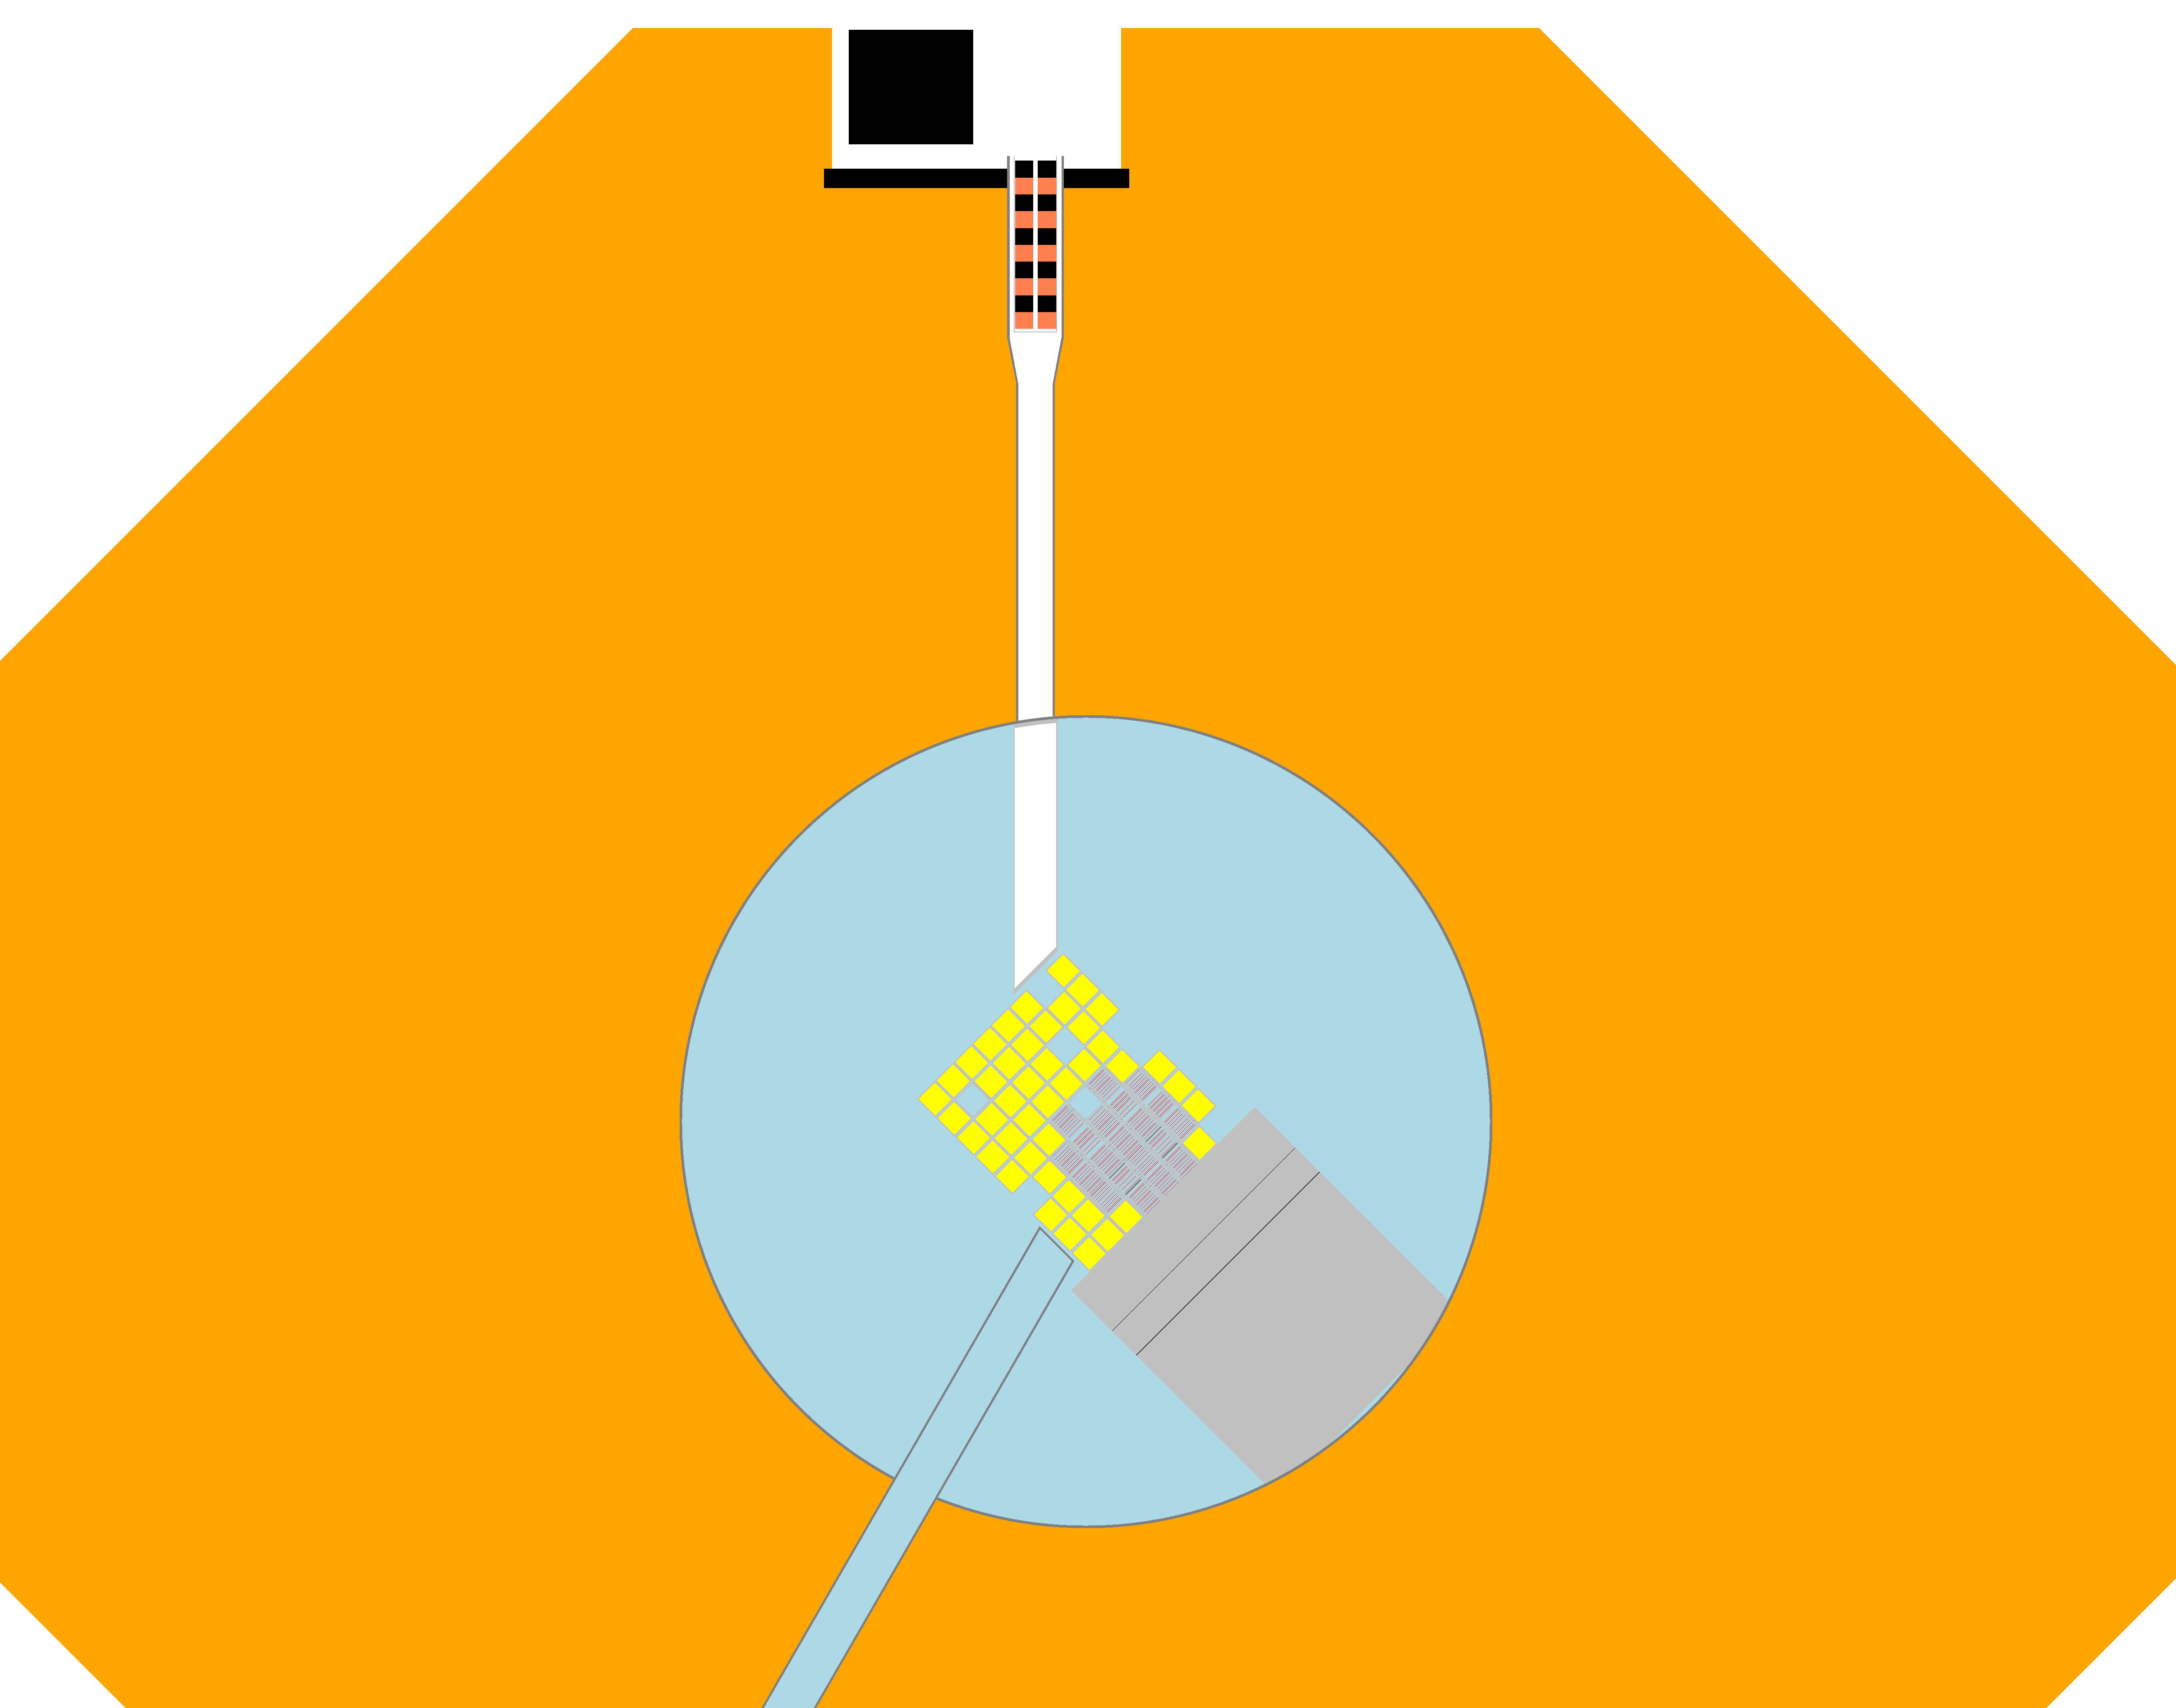
\includegraphics[width=0.75\textwidth]{ra6.png}
\caption{Esquema representativo del núcleo del RA-6. En el mismo se observa la disposición de los elementos combustibles, el conducto Nº1 (inferior) y el conducto Nº5 (superior) \cite{DeptoNeutronesCAB2025}.}
\label{fig:esquema-nucleo}
\end{figure}

El reactor cuenta con cinco conductos de extracción de neutrones destinados a experimentación. En la Figura~\ref{fig:esquema-nucleo} se destacan dos de ellos: el conducto Nº1 y el conducto Nº5. En particular, el conducto Nº5 se orienta hacia una zona del núcleo en la que se encuentran ubicadas un bloque de grafito y un bloque de agua. Dado que no apunta directamente hacia los elementos combustibles, el espectro resultante en este canal está compuesto mayoritariamente por neutrones térmicos.

El conducto Nº5 consiste en un cilindro de acero de 5cm de radio, que atraviesa la pileta del reactor y el blindaje biológico. En su interior se encuentra un colimador constituido por secciones alternadas de plomo y parafina borada. Además, las dos primeras secciones del colimador contienen un filtro de bismuto, utilizado para atenuar la componente de radiación $\gamma$ del haz. Esta atenuación resulta fundamental en experimentos, ya que permite reducir el fondo de radiación $\gamma$ que puede saturar los detectores utilizados. La Figura \ref{fig:conducto} muestra un esquema detallado del conducto Nº5 y de su sistema de colimación, como así también el banco de detectores utilizados en la medición experimental.

\begin{figure}[h]
\centering
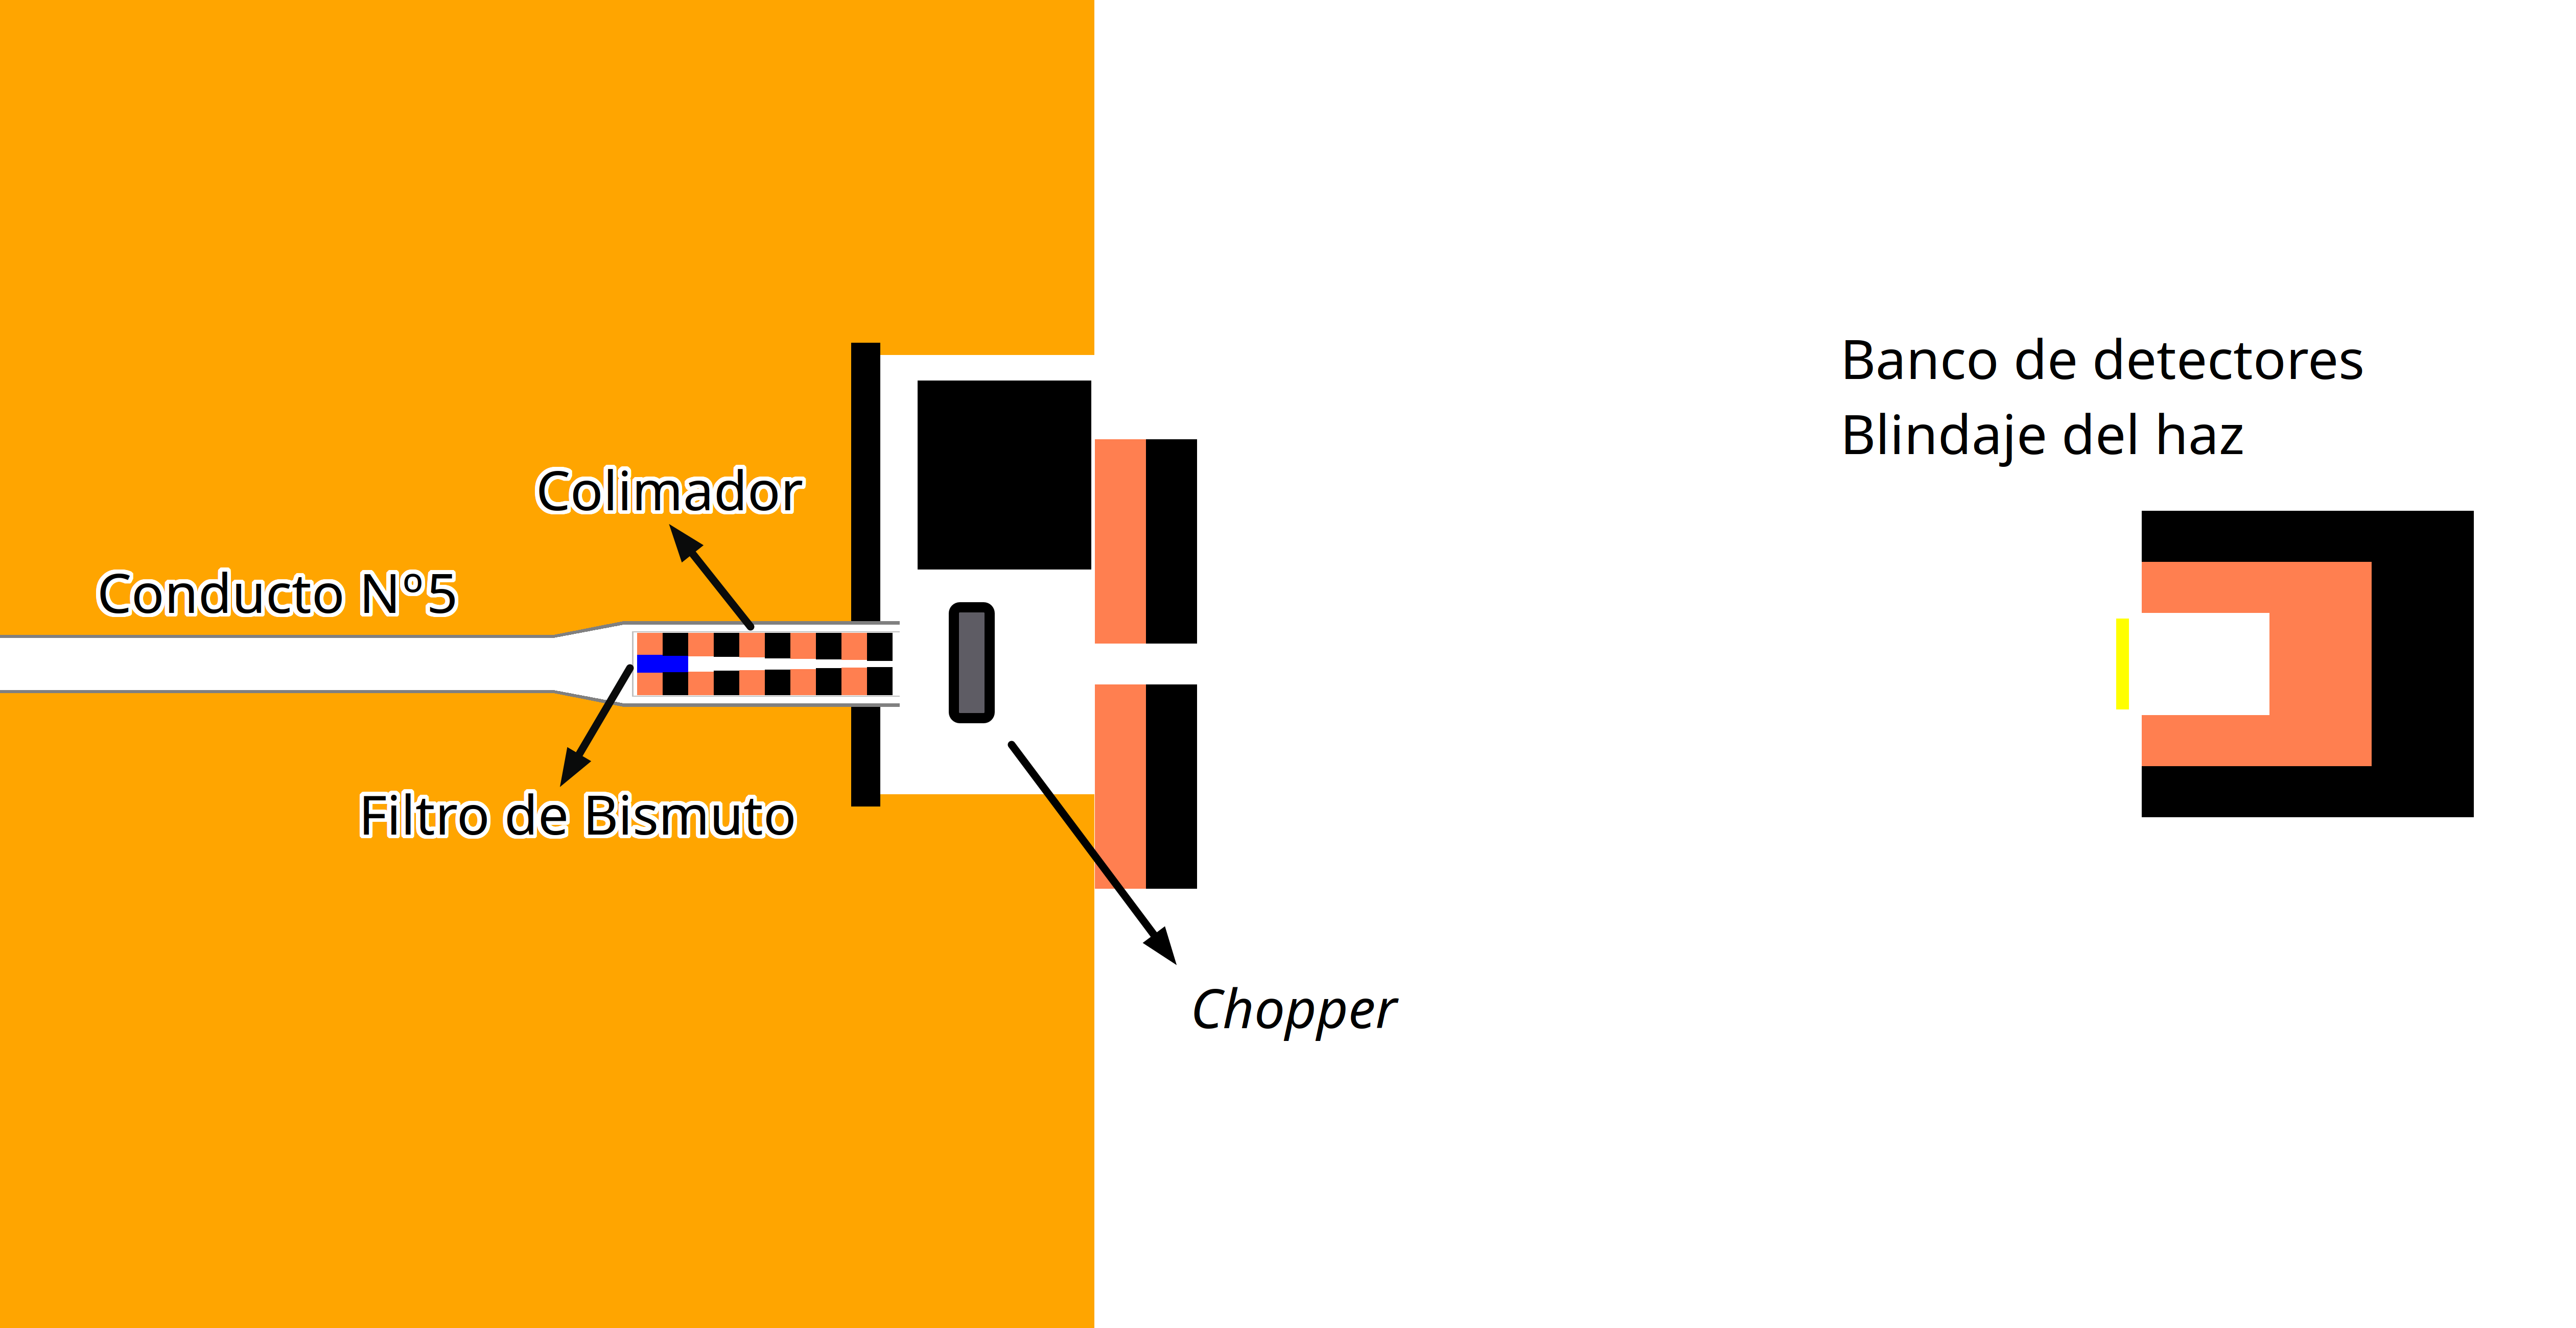
\includegraphics[width=0.9\textwidth]{conducto.png}
\caption{Esquema representativo del conducto Nº5 del RA-6 y de la instalación experimental asociada al \textit{chopper} \cite{DeptoNeutronesCAB2025}.}
\label{fig:conducto}
\end{figure}

Este conducto está asociado a un intrumento experimental denominado \textit{chopper}, diseñada para la generación de haces pulsados de neutrones. El dispositivo \textit{chopper} consiste en un disco rotatorio de material absorbente con una ranura, el cual se posiciona a la salida del conducto. Al girar a velocidad constante, la ranura permite periódicamente el paso de neutrones cuando se encuentra alineada con el eje del haz. De esta manera, se obtienen pulsos neutrónicos que pueden ser utilizados para realizar espectrometría mediante la técnica de tiempo de vuelo (TdV). La Figura \ref{fig:chopper} ilustra esquemáticamente el mecanismo de funcionamiento del disco \textit{chopper}.

\begin{figure}[h]
\centering
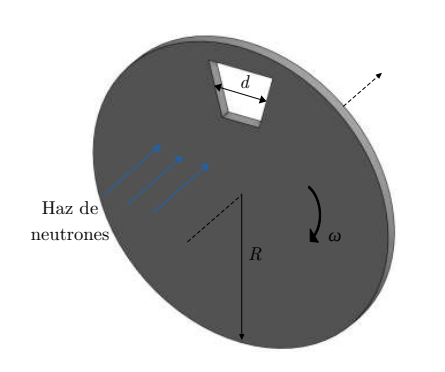
\includegraphics[width=0.5\textwidth]{DISCO_CHOPPER.png}
\caption{Esquema representativo del disco rotatorio del \textit{chopper} empleado en el conducto Nº5. La ranura permite el paso periódico de neutrones, generando un haz pulsado \cite{DeptoNeutronesCAB2025}.}
\label{fig:chopper}
\end{figure}

Para la implementación experimental de esta técnica, se dispone un banco de cinco detectores de \textsuperscript{3}He a una distancia conocida de la salida del conducto. Estos detectores registran el tiempo de llegada de cada neutrón, a partir del cual se calcula su energía cinética mediante la expresión:

\begin{equation}
E = \frac{1}{2} m_n v^2,
\end{equation}

donde $E$ es la energía del neutrón, $m_n$ su masa, y $v$ la velocidad obtenida como el cociente entre la distancia conocida y el tiempo medido.

Para reconstruir correctamente el espectro neutrónico, es necesario corregir la señal detectada. En primer lugar, se debe restar un fondo constante asociado a la componente gamma y a neutrones que atraviesan el \textit{chopper} fuera de fase. Adicionalmente, se aplican correcciones por el tiempo muerto del sistema de adquisición de datos y por la eficiencia de detección de los tubos de \textsuperscript{3}He.

Finalmente, detrás del banco de detectores se instala un blindaje adicional que permite blindar el haz y proteger las áreas experimentales circundantes.

\section{Procesamiento del archivo de partículas}

% El departamento de neutrones del CAB ha proporcionado un archivo de partículas que contiene información sobre las trayectorias de los neutrones que ingresan al conducto N5. Este archivo surge de una simulacion desde nucleo del RA-6 en OpenMC. Esta simulacion consto de 1e10 particulas, y se registro un archivo de particulas que contenia 41245 particulas que ingresaron al conducto N5. Sin embargo como estas particulas provienen de una simulacion con esquema de reduccion de varianza incorporado, algunas de estas particulas tienen un peso menor a 1. Por lo tanto, en el archivo de particulas original se cuenta con un total de 22182 de peso estadistico, sumando todas las particulas. 

% En la figura tal se presenta la distribucion en el plano XY de las particulas. Estas forman un circulo de radio $5,\text{cm}$, que corresponde al radio del conducto. Se observa que las particulas se distribuyen uniformemente en el circulo.

% \begin{figure}[h]
%     \centering
%     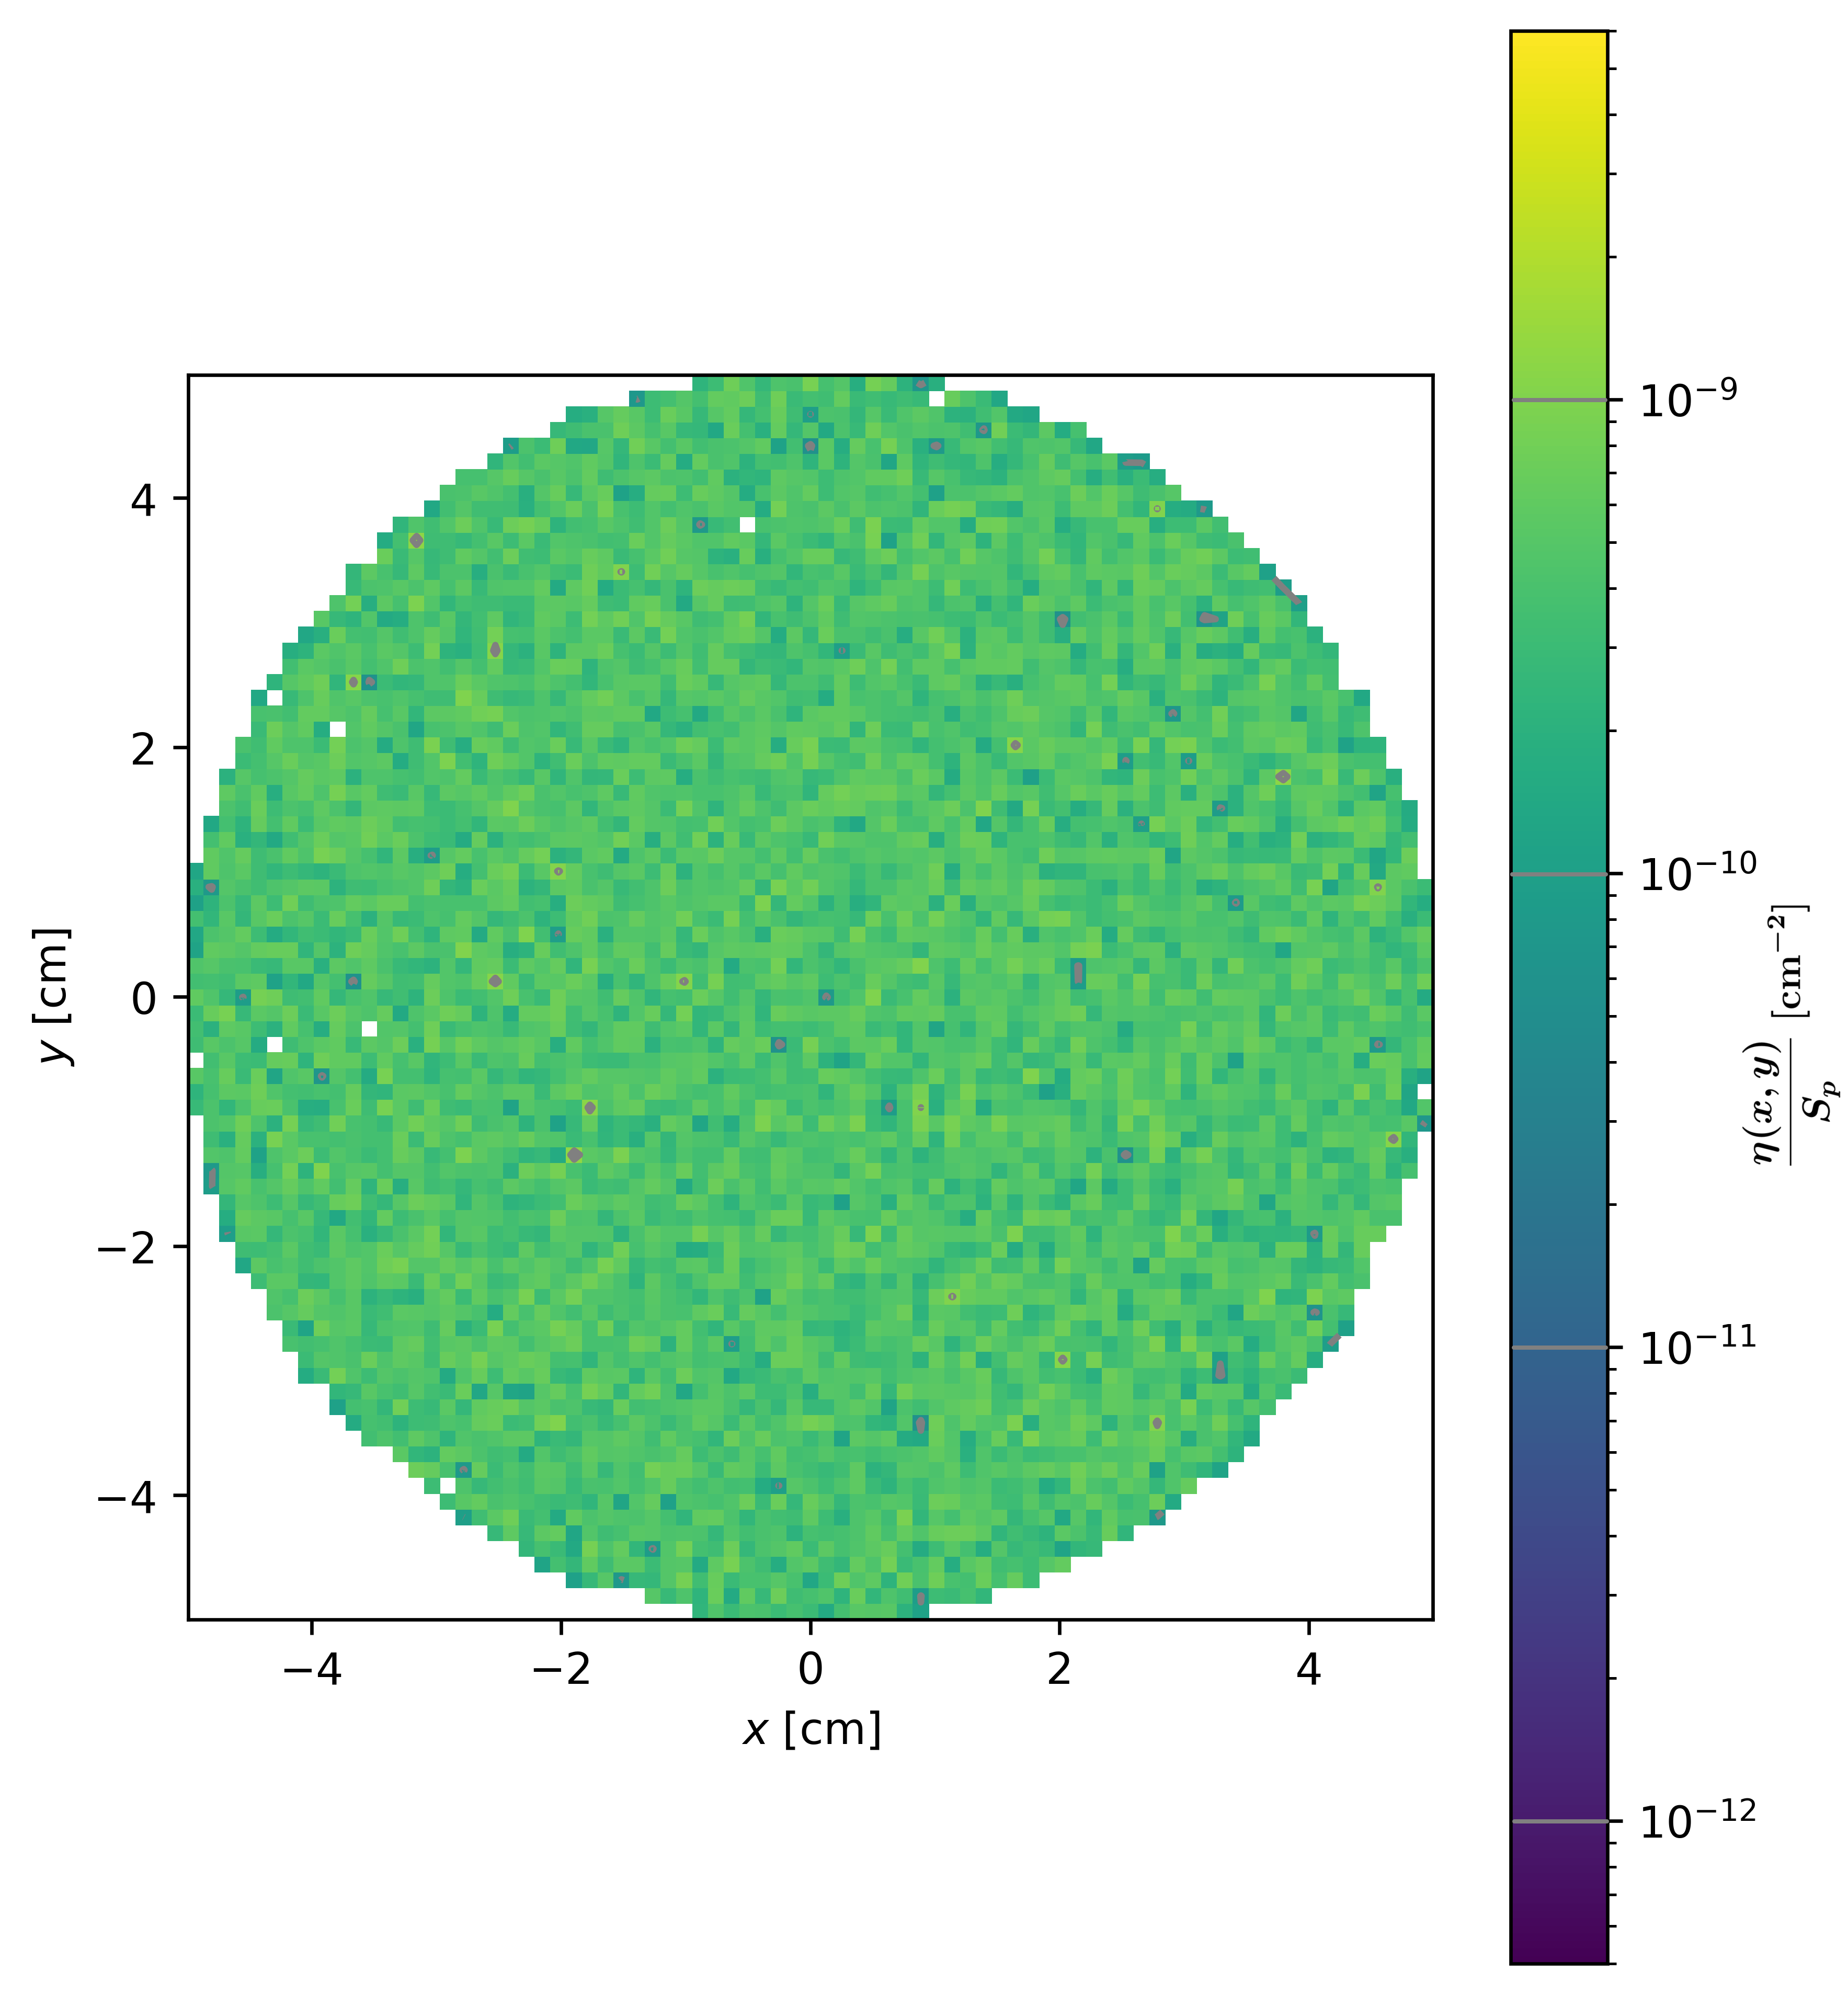
\includegraphics[width=0.75\textwidth]{conducto_XY.png}
%     \caption{Distribución espacial de las partículas del archivo original en el plano XY.}
%     \label{fig:conducto-XY}
% \end{figure}

% En la figura tal se presenta la distribucion de letargia de las particulas del archivo original. Se observa que las mismas presentan una acumulacion sobre la region de fision alrededor de $ln(E_0/E) = 2$, donde $E_0 = 20 MeV$ y otra acumulacion de mayor proporsion en la region de termalizacion alrededor de $ln(E_0/E) = 19$.

% \begin{figure}[h]
%     \centering
%     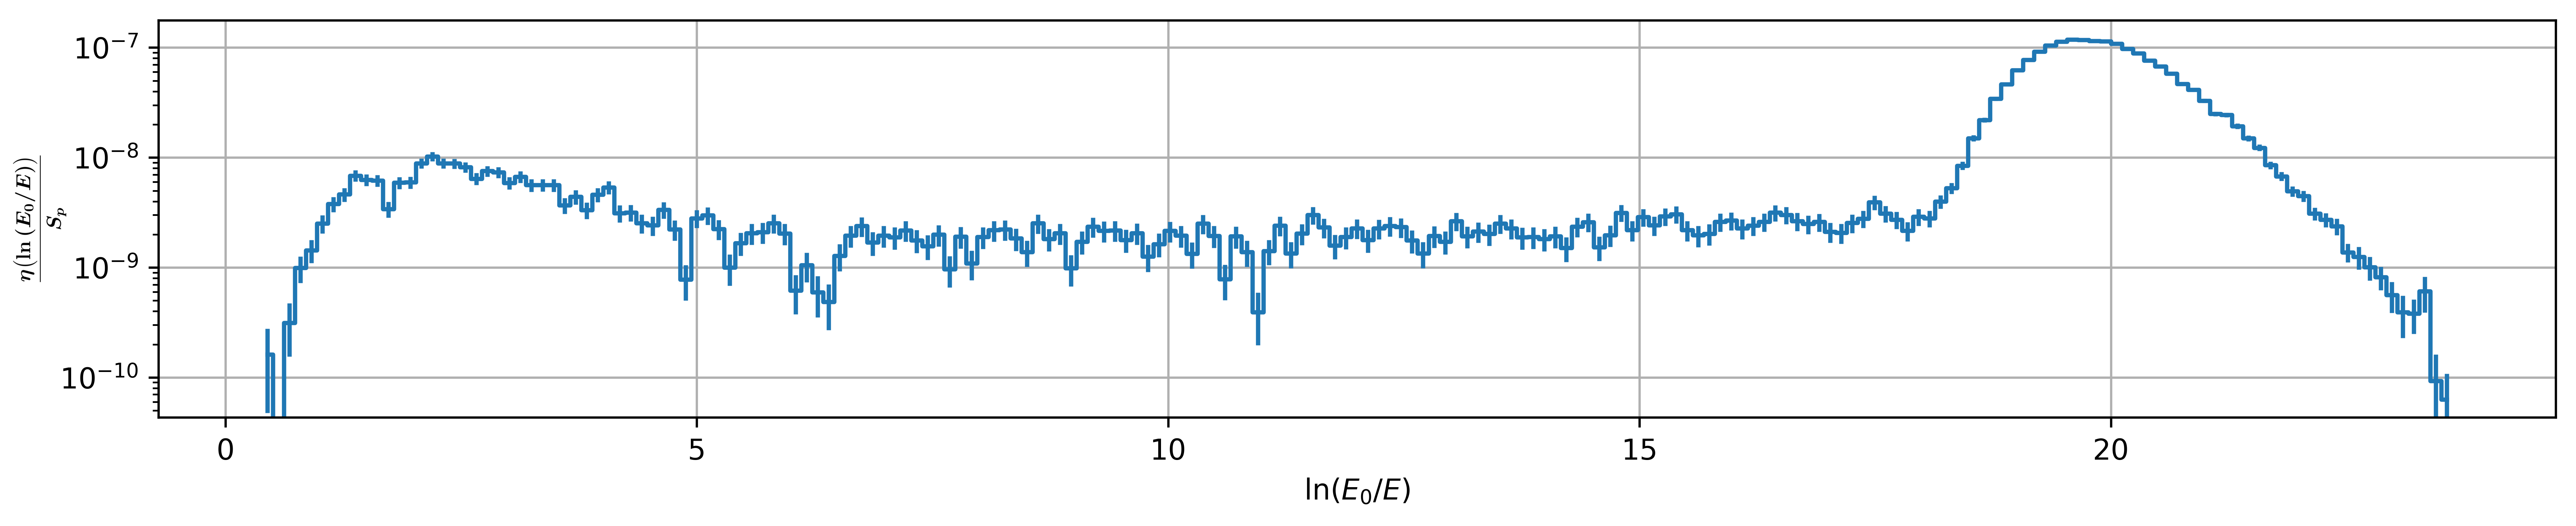
\includegraphics[width=\textwidth]{conducto_let.png}
%     \caption{Distribución de letargía de las partículas del archivo original.}
%     \label{fig:conducto-let}
% \end{figure}

% Para generar la fuente distribucional, se emplea el método de histogramas multidimensionales desarrollado en este trabajo. La configuracion utilizada fue:


% \begin{itemize}
%     \item Orden de procesamiento: \texttt{[letargía, X, Y, $\mu$, $\phi$]}
%     \item Número de histogramas macro: [3, 7, 4, 4]
%     \item Número de histogramas micro: [75, 18, 18, 15, 10]
% \end{itemize}

% Se decidio brindarle mayor resolucion a la letargia, ya que es la variable de mayor interes en este caso y es necesario obtener una buena resolucion en la zona de termalizacion, debido a que el objetivo de este capitulo es comparar el espectro termico medido a traves de la tecnica de TdV. 

% A su vez se decidio brindarle la mayor cantidad de bines al histograma macro de la variable $X$ para obtener una mejor representacion del circulo. En caso de tomar menos bines para la variable $X$ se observaria patrones debidos a la discretizacion del histograma macro.

% Con esta fuente distribucional se procede a comparar el resultado obtenido de las distribuciones de letargia y posicion XY de las particulas. En la figura tal se presenta la distribucion en el plano XY de las particulas generadas por la fuente distribucional. A comparacion con la otra figura se observa que se logra representativomente el circulo de radio $5,\text{cm}$, aunque sin embargo se pueden apreciar los bordes debidos a la discretizacion con histogramas macro aplicada.

% \begin{figure}[h]
%     \centering
%     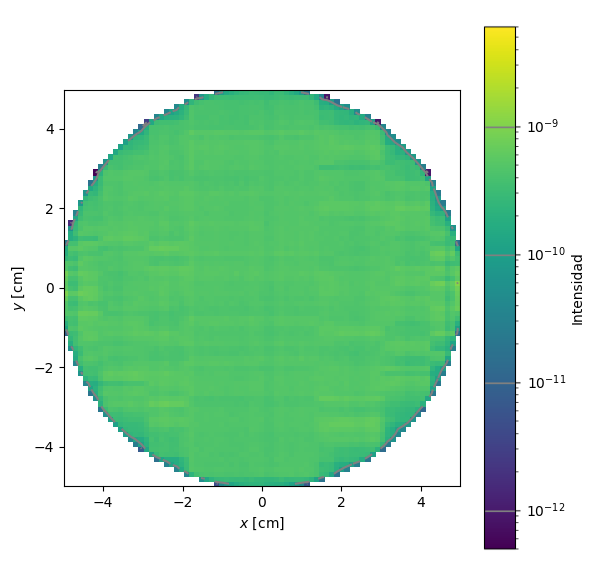
\includegraphics[width=0.75\textwidth]{conducto_comparacion_XY.png}
%     \caption{Distribución espacial de las partículas de la fuente distribucional en el plano XY.}
%     \label{fig:conducto-comparacion-XY}
% \end{figure}

% En la figura tal se presenta la comparacion de la distribucion de letargia de las particulas del archivo original y las generadas por la fuente distribucional. Se observa la mayor resolucion en el histograma de letargia, para poder obtener una aproximacion de mejor resolucion en la zona de termalizacion, a costa de reproducir el ruido estadistico en la zona epitermica.

% \begin{figure}[h]
%     \centering
%     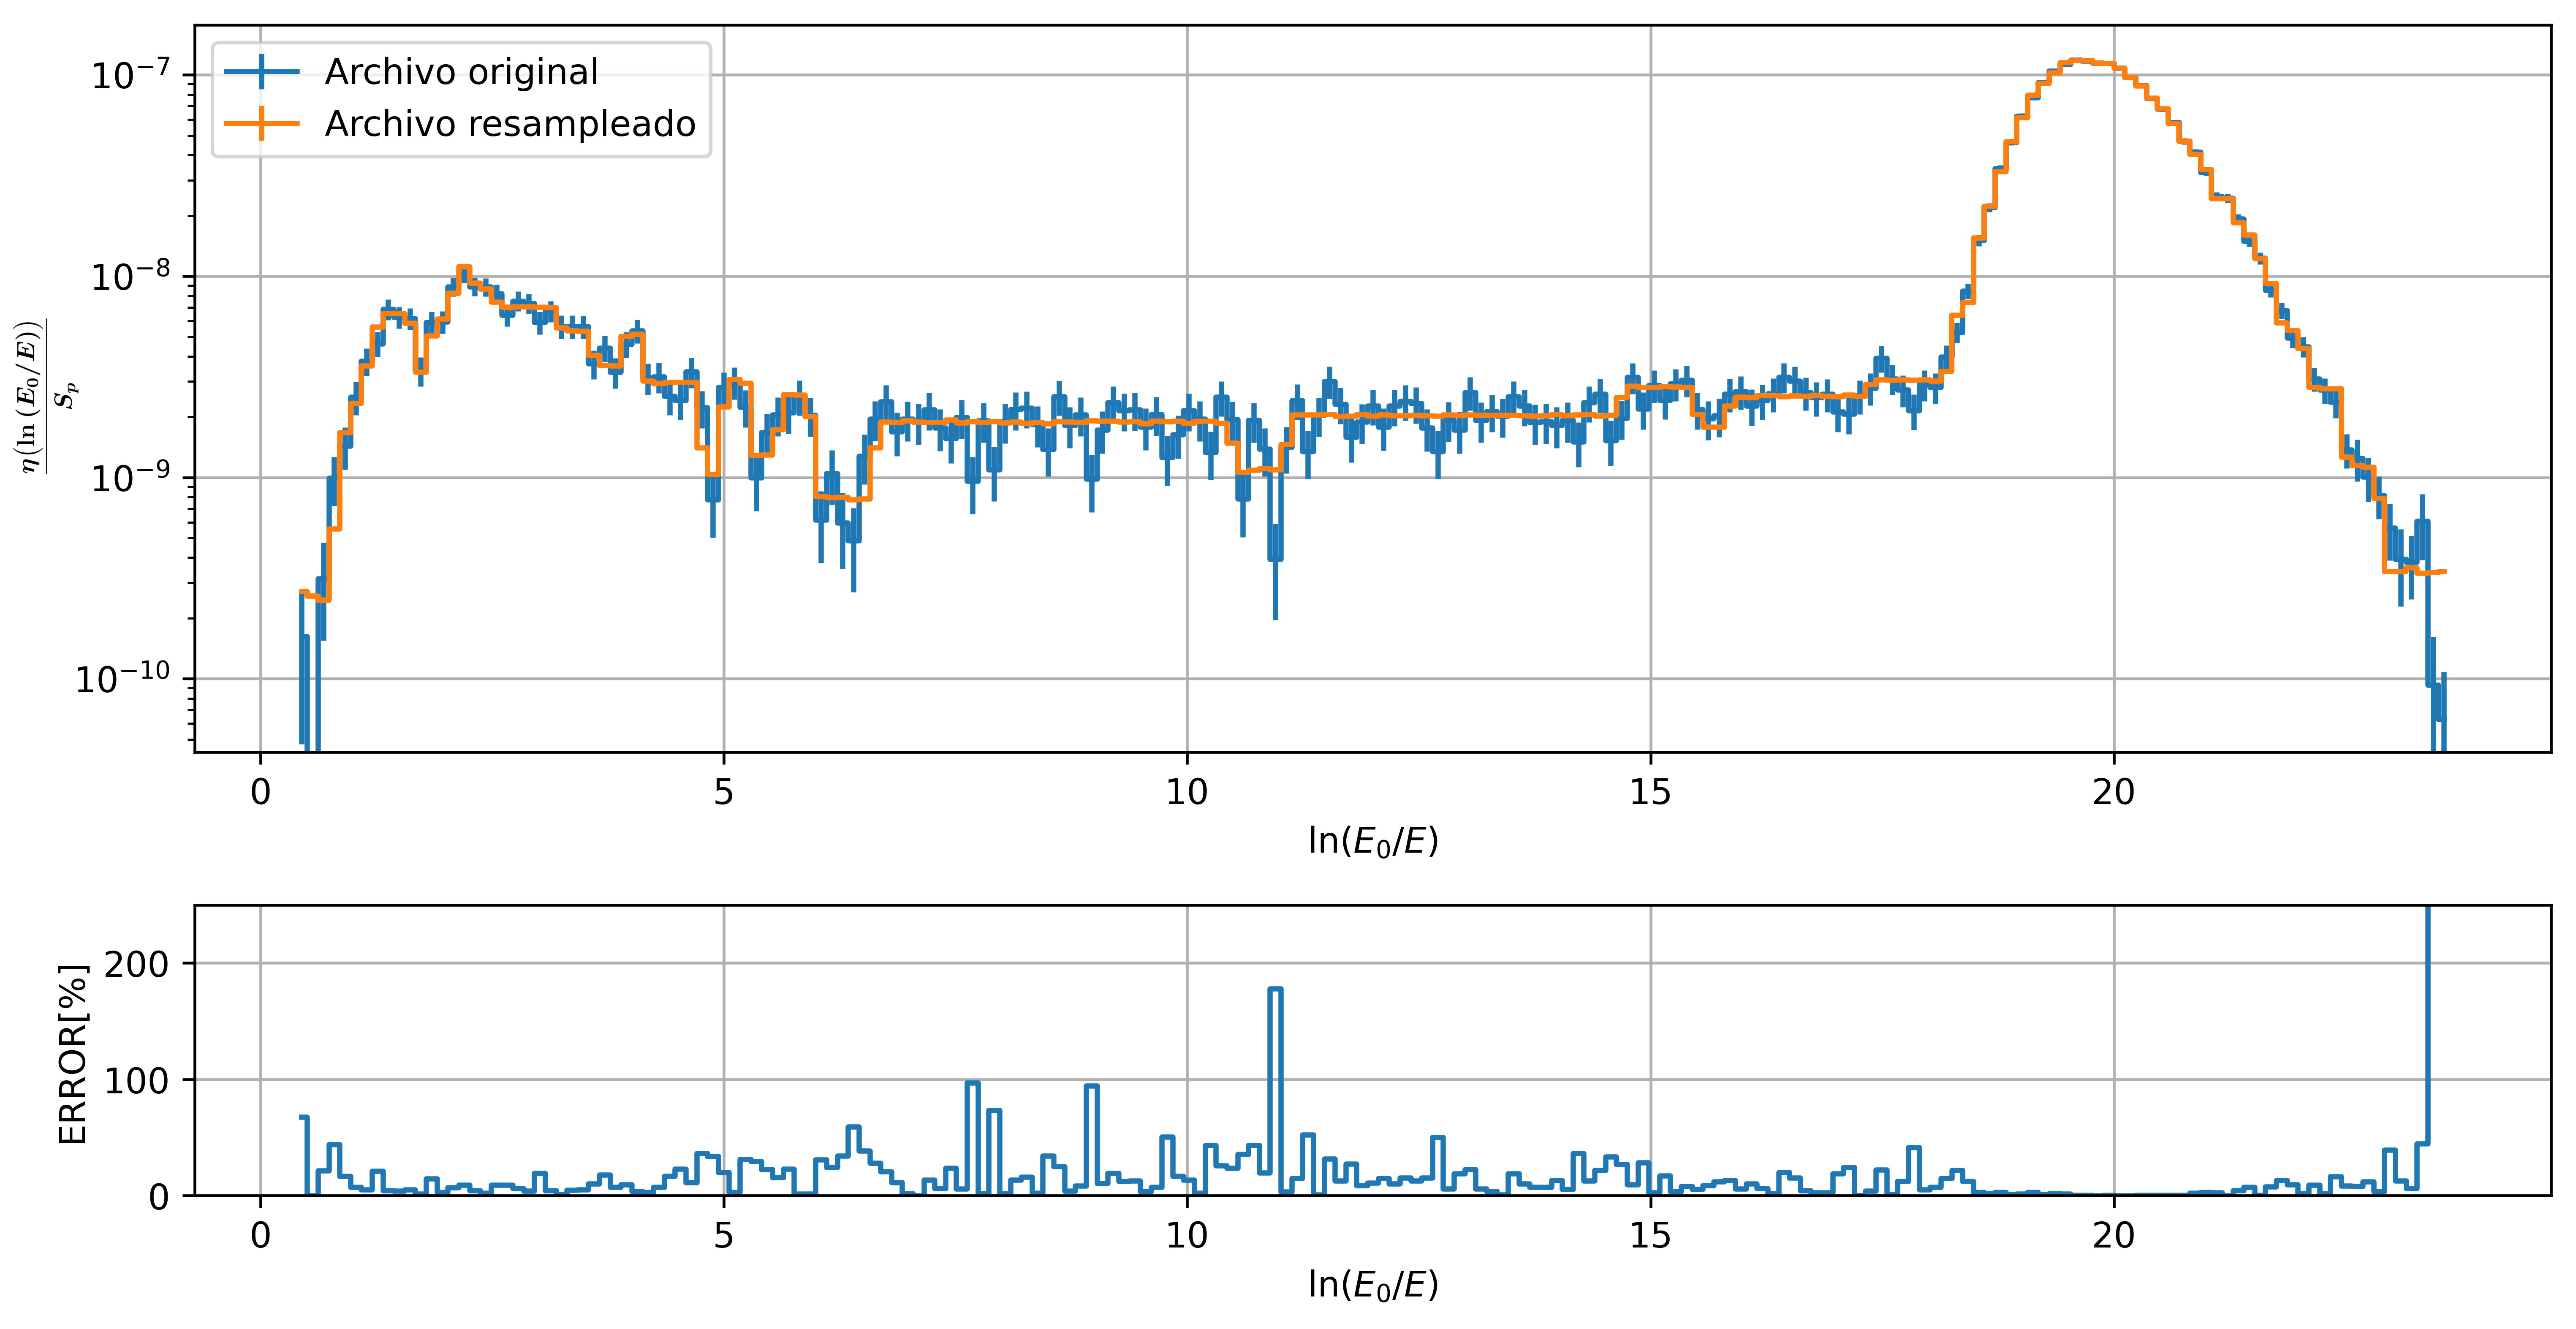
\includegraphics[width=\textwidth]{conducto_comparacion_let.png}
%     \caption{Comparación de la distribución de letargia entre el archivo original y la fuente distribucional.}
%     \label{fig:conducto-comparacion-let}
% \end{figure}

El Departamento de Neutrones del Centro Atómico Bariloche proporcionó un archivo de partículas que contiene información sobre los neutrones que ingresan al conducto Nº5. Este archivo fue generado a partir de una simulación del núcleo completo del reactor RA-6 utilizando el código \texttt{OpenMC}. La simulación consistió en un total de $10^{10}$ partículas fuente, de las cuales 41245 fueron registradas en la entrada del conducto Nº5.

Cabe destacar que esta simulación fue realizada con un esquema de reducción de varianza, lo que implica que muchas partículas del archivo presentan un peso estadístico menor a la unidad. La suma total de los pesos estadísticos de las partículas registradas fue 22182.

En la Figura~\ref{fig:conducto-XY} se muestra la distribución espacial de las partículas registradas en el plano $XY$. Puede observarse que las posiciones conforman un círculo de radio 5~cm, correspondiente a la sección transversal del conducto Nº5. La distribución es aproximadamente uniforme dentro del círculo.

\begin{figure}[h]
\centering
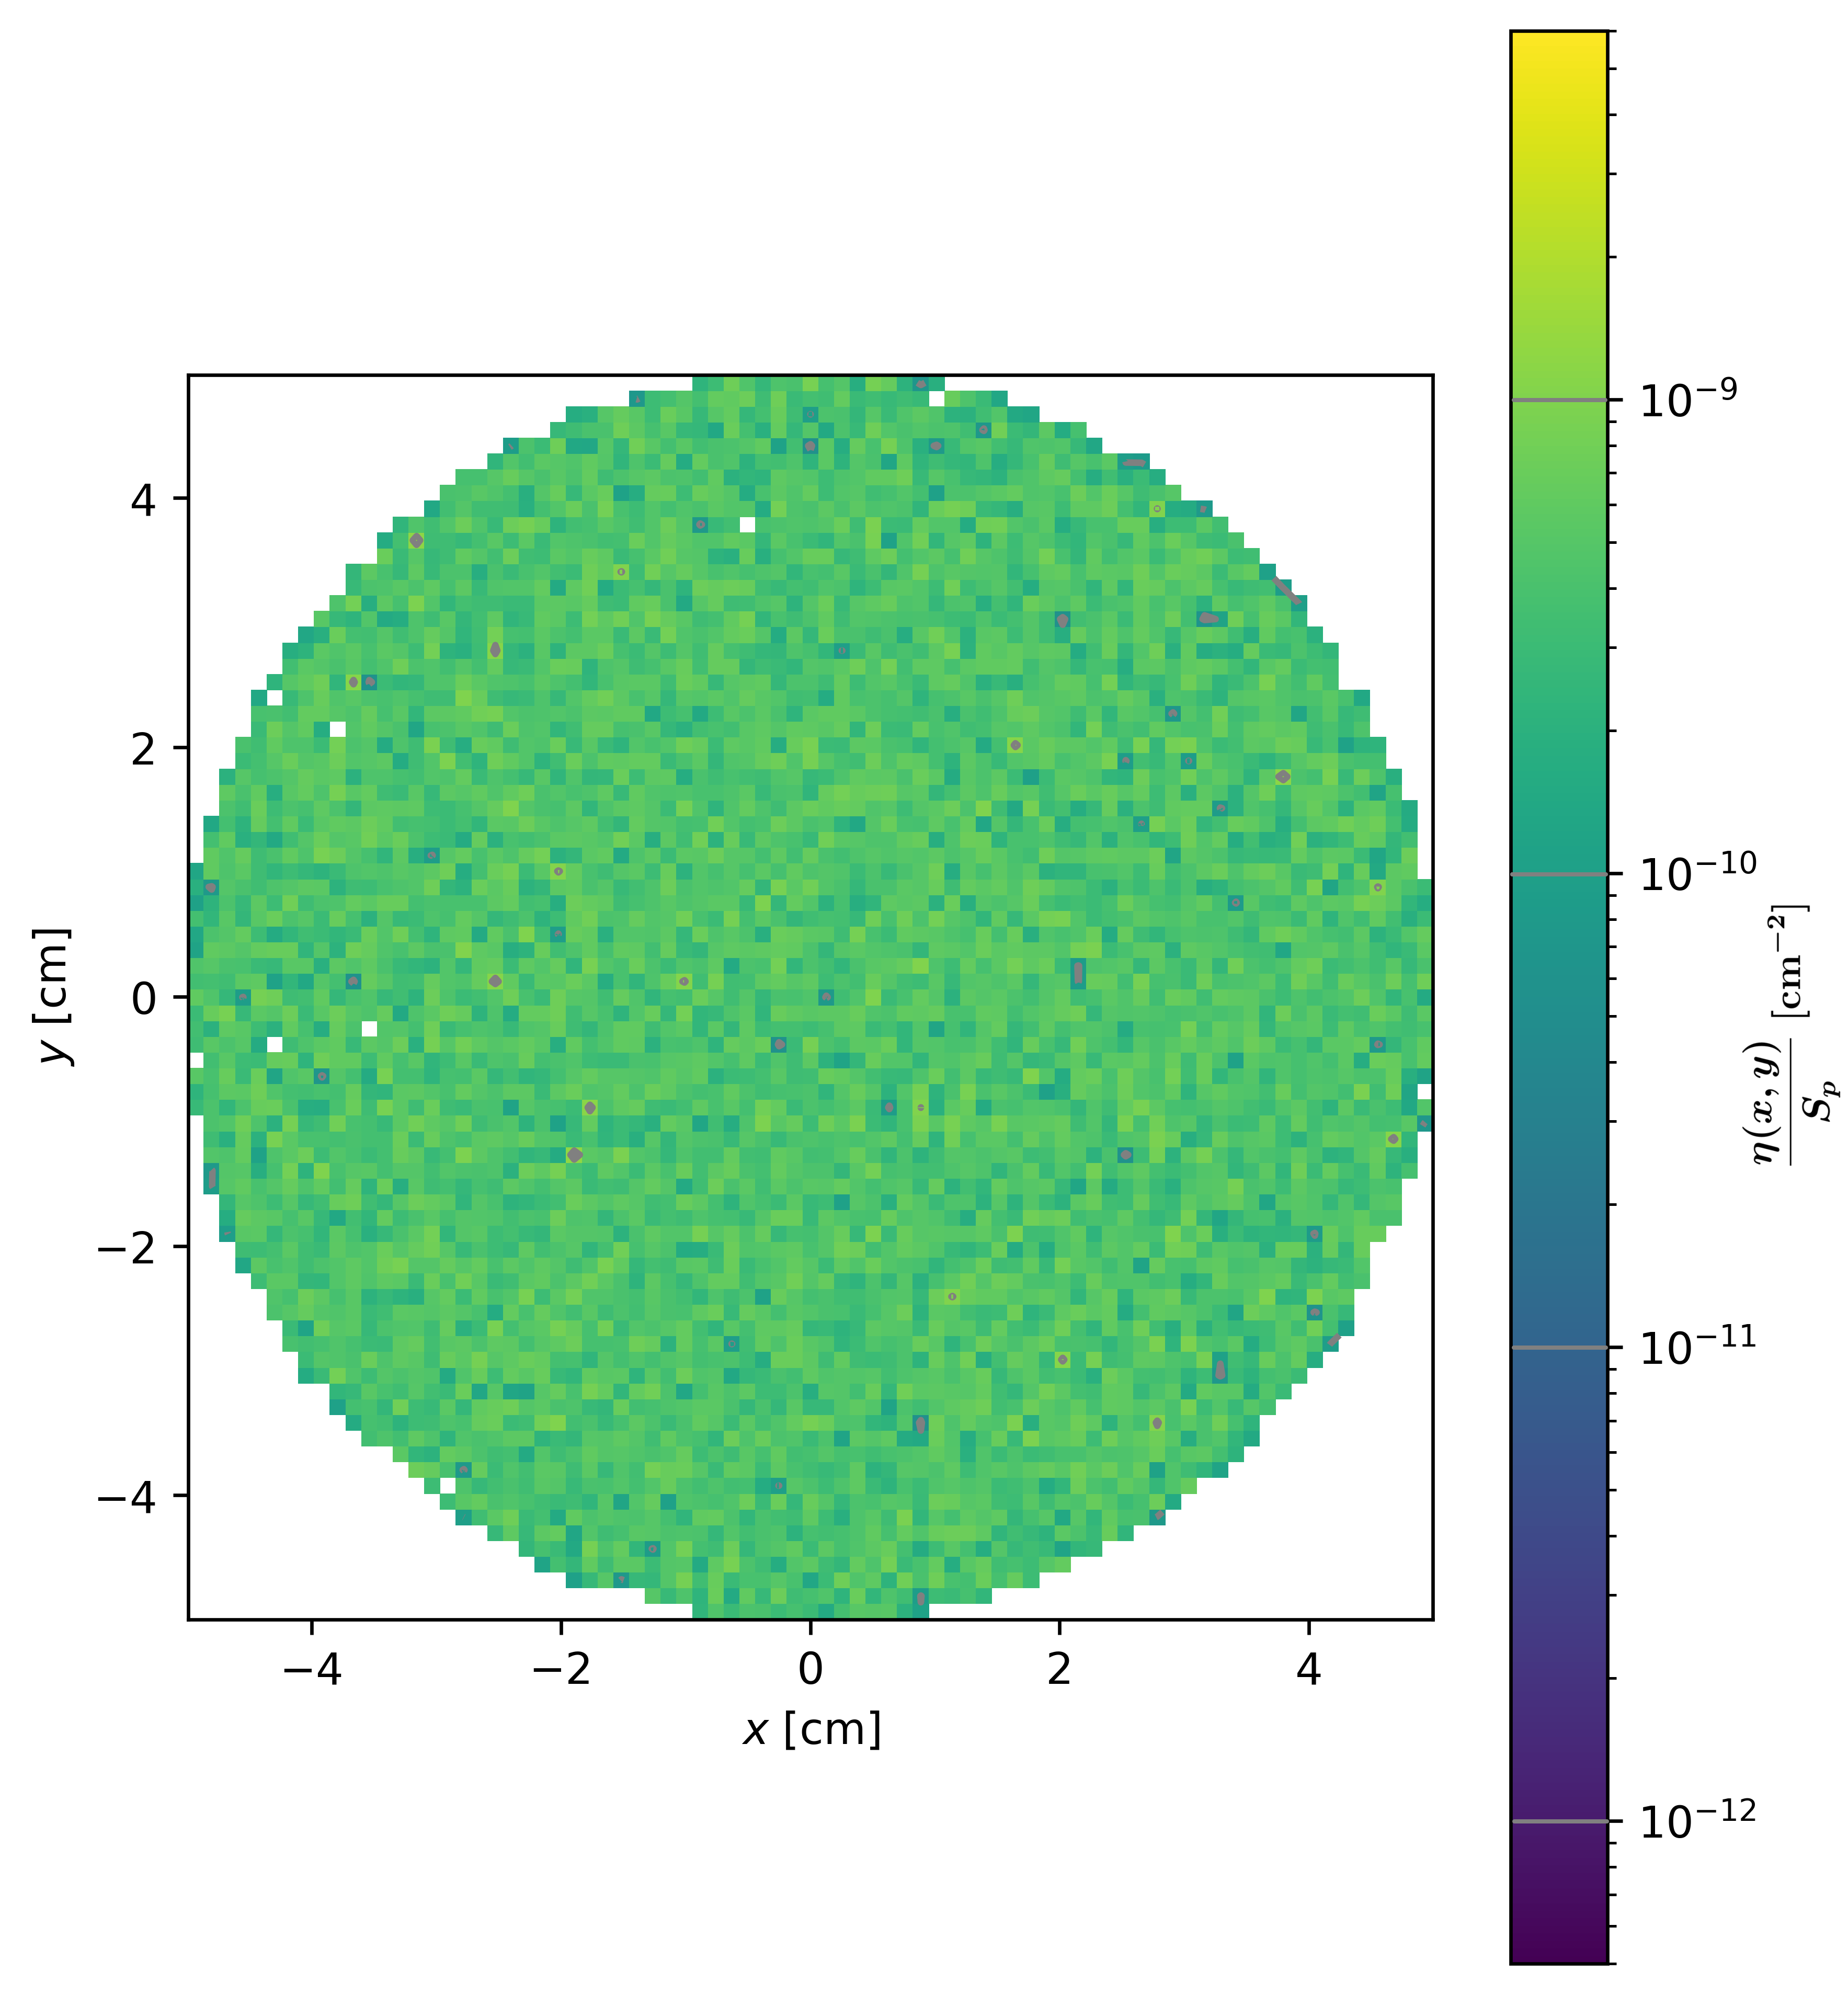
\includegraphics[width=0.75\textwidth]{conducto_XY.png}
\caption{Distribución espacial de las partículas del archivo original en el plano $XY$.}
\label{fig:conducto-XY}
\end{figure}

La Figura~\ref{fig:conducto-let} presenta la distribución de letargía de las partículas registradas. Se observan dos regiones de acumulación: una alrededor de $\ln(E_0/E) \approx 2$, correspondiente a energías típicas de fisión, y otra de mayor intensidad en la región térmica, centrada en $\ln(E_0/E) \approx 19$, donde $E_0 = 20$~MeV.

\begin{figure}[h]
\centering
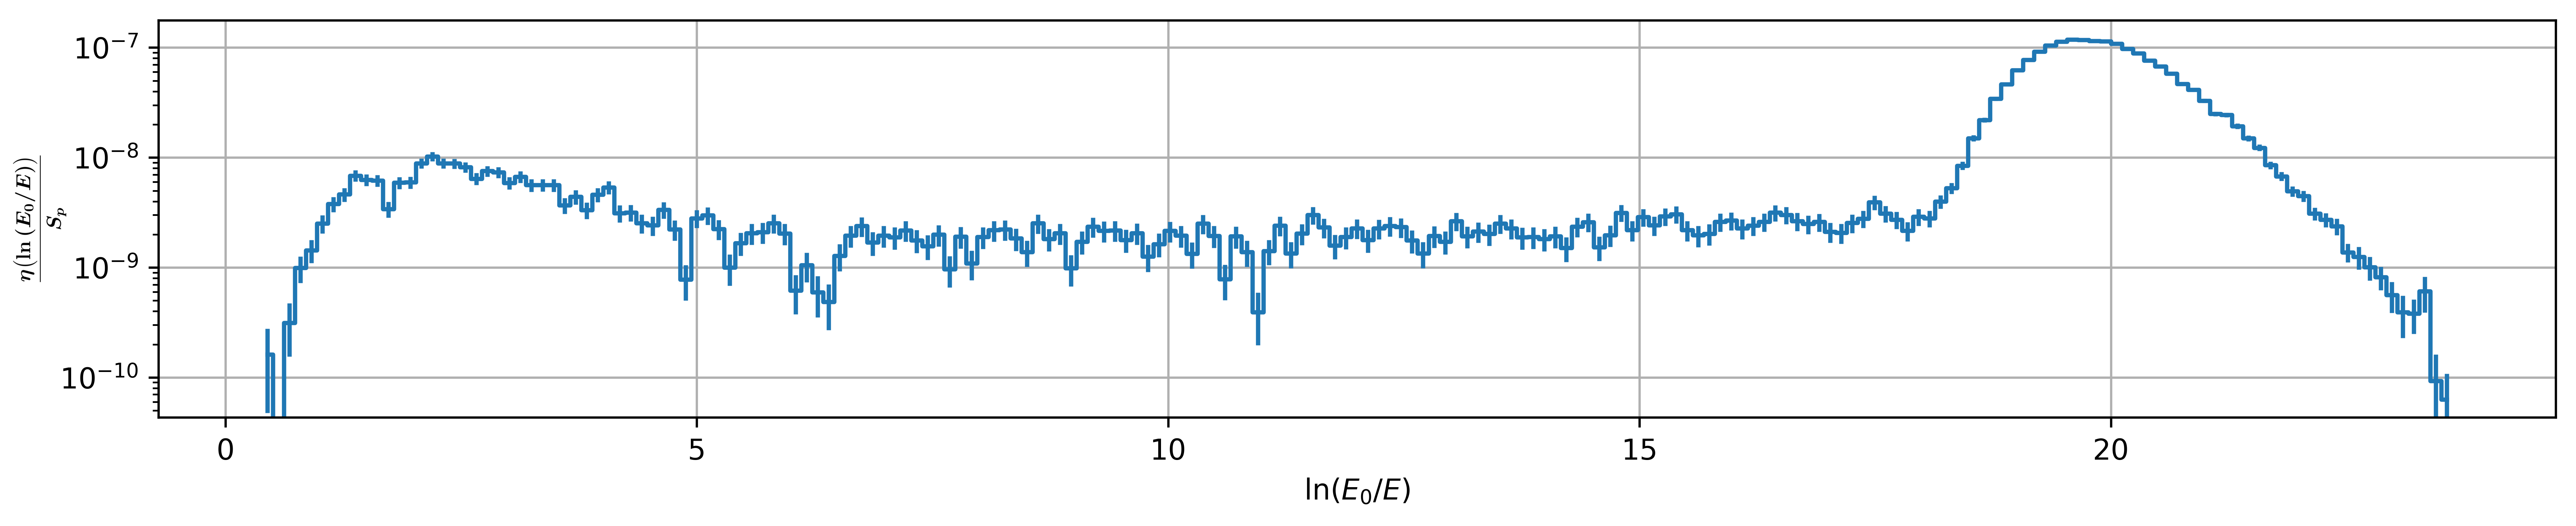
\includegraphics[width=\textwidth]{conducto_let.png}
\caption{Distribución de letargía de las partículas del archivo original.}
\label{fig:conducto-let}
\end{figure}

A partir de este archivo de partículas, se generó una fuente distribucional mediante el método de histogramas multidimensionales desarrollado en este trabajo. La configuración adoptada para la construcción de la fuente distribucional fue la siguiente:

\begin{itemize}
\item \textbf{Orden de procesamiento}: \texttt{[letargía, X, Y, $\mu$, $\phi$]}
\item \textbf{Número de histogramas macro}: \texttt{[3, 7, 4, 4]}
\item \textbf{Número de histogramas micro}: \texttt{[75, 18, 18, 15, 10]}
\end{itemize}

Se asignó una mayor resolución a la variable letargía, dado que constituye el objetivo principal de análisis en este capítulo, centrado en la comparación espectral mediante la técnica de tiempo de vuelo. Además, se destinó una mayor cantidad de divisiones macro a la coordenada $X$ para mejorar la representación del contorno circular del conducto. Se verificó que al reducir la resolución en dicha coordenada, aparecían patrones discretos artificiales en el plano $XY$, producto de una segmentación insuficiente del dominio espacial.

La Figura~\ref{fig:conducto-comparacion-XY} muestra la distribución en el plano $XY$ de las partículas generadas por la fuente distribucional. Puede observarse que la forma circular de radio 5~cm se reproduce adecuadamente, aunque la discretización asociada a los histogramas macro introduce estructuras visibles en los bordes.

\begin{figure}[h]
\centering
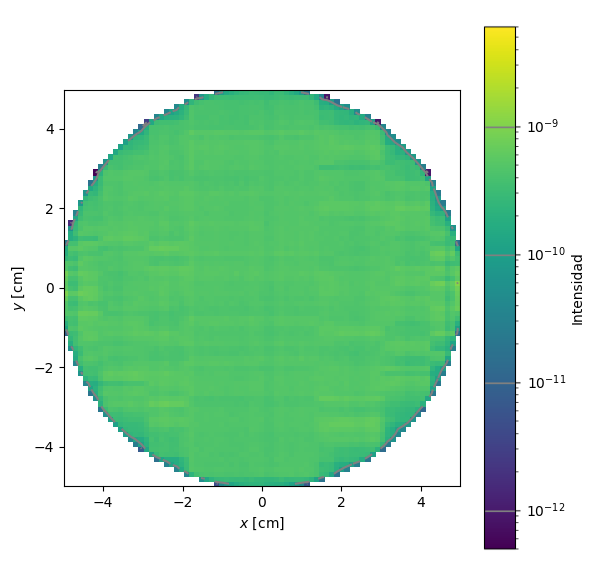
\includegraphics[width=0.75\textwidth]{conducto_comparacion_XY.png}
\caption{Distribución espacial de las partículas de la fuente distribucional en el plano $XY$.}
\label{fig:conducto-comparacion-XY}
\end{figure}

En la Figura~\ref{fig:conducto-comparacion-let} se presenta la comparación entre la distribución de letargía del archivo original y la correspondiente a la fuente generada. La mayor resolución elegida para el eje de letargía permite representar en detalle la zona térmica, a costa de reproducir parte del ruido estadístico presente en la región epitérmica.

\begin{figure}[h]
\centering
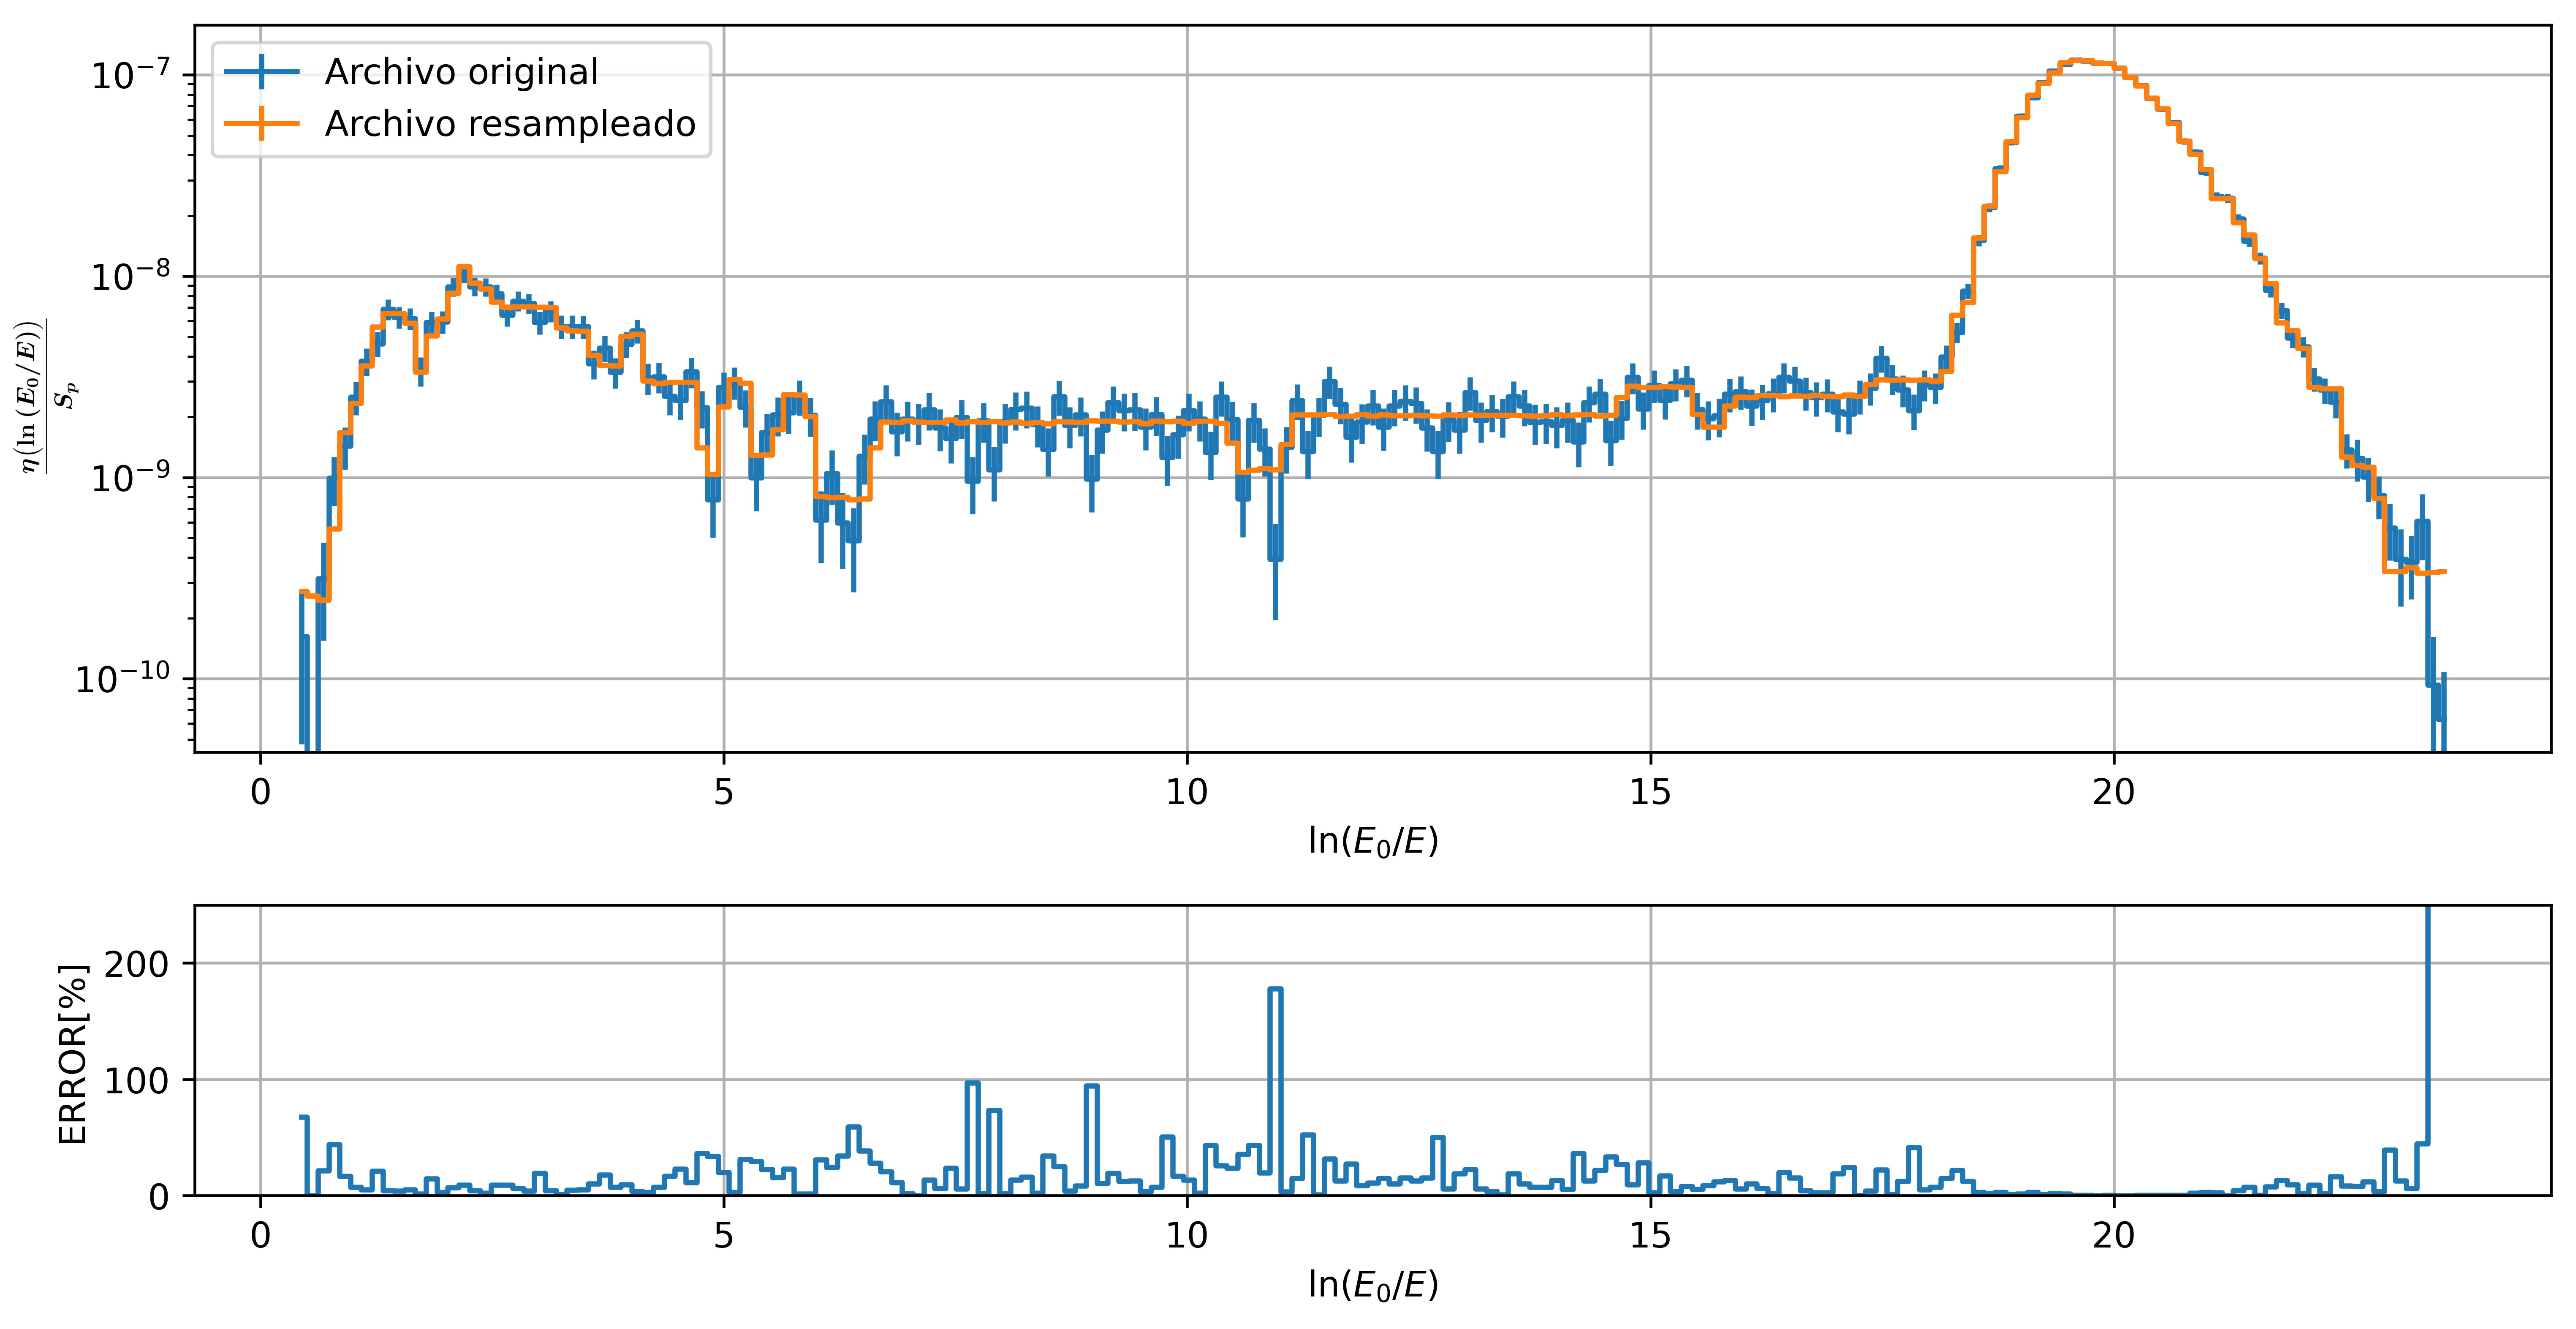
\includegraphics[width=\textwidth]{conducto_comparacion_let.png}
\caption{Comparación de la distribución de letargía entre el archivo original y la fuente distribucional.}
\label{fig:conducto-comparacion-let}
\end{figure}

% \label{sec:optimizacion-w}

\section{Resultados de simulación en \texttt{OpenMC} y comparación experimental}
% \label{sec:resultados-w}

% A partir de la fuente distribucional generada, se procedio a hacer una segunda simiulacion del conducto N5, esta vez utilizando la fuente generada por el método de remuestreo. Esta simulacion consto de 5e9 particulas. Para aumentar la estadistica se utilizo un esqeuam de reduccion de varianza de tipo sesgo de supervivencia, que permite aumentar la probabilidad de que las particulas lleguen al banco de detectores.

% En esta simulacion se registro el flujo neutronico en todo el modelo y se registro el espectro neutronico obtenido en el banco de detectores. Este espectro neutronico se comparo contra el espectro medido experimentalmente en el N5 por tecnica de TdV. 

% \subsection{Distribución espacial del flujo}
% En la figura tal se presenta el flujo neutronico obtenido en el modelo implementado del conducto N5. Se observa que se ha adquirido un flujo converjido en la zona del banco de detectores. Tambien es posible observar que el flujo decae varios ordenes de magnitud al atravesar el conducto y el colimador. Esto evidencia la necesidad de desacoplar la simulacion del conducto del núcleo del reactor, debido a que la probabilidad de que los neutrones lleguen al banco de detectores es muy baja. Por lo tanto en caso de simular desde el nucleo se obtendria que la probabilidad de que lleguen del nucleo al conducto es baja y habria que juntar eso con la probabilidad de que los neutrones atraviesen el colimador y lleguen al banco de detectores, lo que haria que la estadistica en el banco de detectores sea muy baja. En cambio, al desacoplar la simulacion del conducto del nucleo, se logra obtener una estadistica mucho mayor en el banco de detectores, ya que se simula directamente desde la fuente distribucional.

% \begin{figure}[h]
%     \centering
%     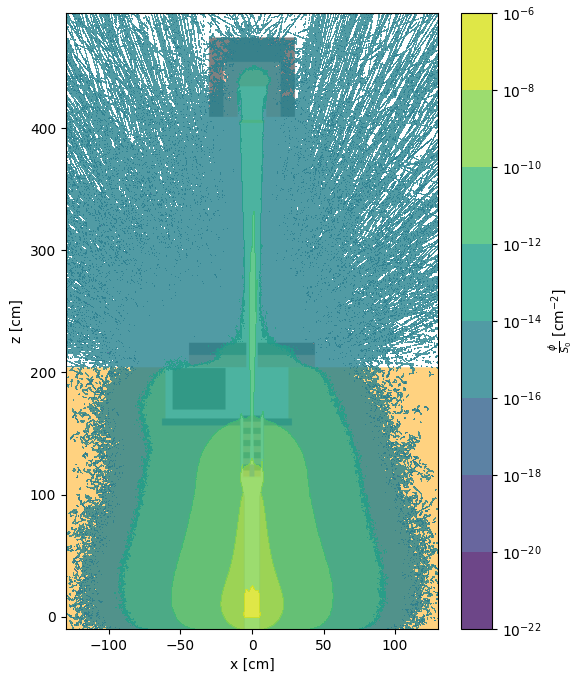
\includegraphics[width=\textwidth]{conducto_flujo.png}
%     \caption{Distribución del flujo neutronico en el modelo del conducto N5.}
%     \label{fig:conducto-flujo}
% \end{figure}

% \subsection{Comparación detector \textsuperscript{3}He}
% En la figura tal se presenta el espectro de neutrones obtenido en el banco de detectores, comparado contra la medicion experimental. Se observa corcordancia entre el espectro medido y el simulado a traves de la fuente distribcuional a partir de los 0.01 eV. Sin embargo, a energias menores a 0.01 eV se observa que el flujo simulado es menor que el medido experimentalmente. 

% \begin{figure}[h]
%     \centering
%     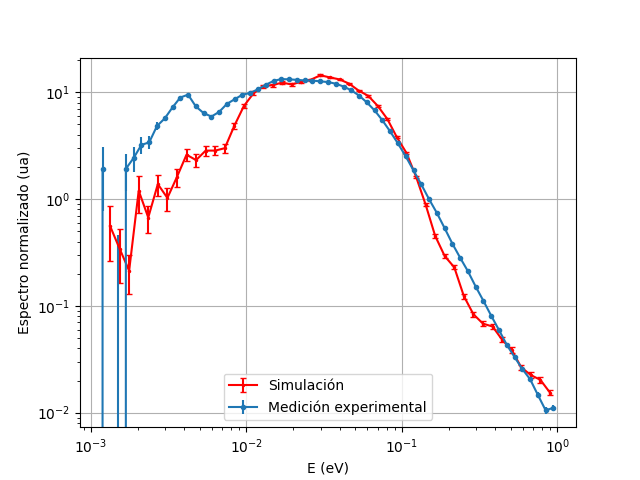
\includegraphics[width=\textwidth]{conducto_espectro.png}
%     \caption{Comparación del espectro de neutrones obtenido en el banco de detectores en la simulación de \texttt{OpenMC} con la medición experimental realizada por TdV por el Departamento de Neutrones del CAB.}
%     \label{fig:conducto-espectro}
% \end{figure}

% Esta discrepancia puede deberse a dos razones:
% \begin{itemize}
%     \item En la figura de la comparacion de letargia se observa que en la zona de mayor letargia se presenta mayor discrepancia entre el espectro del archivo original y el espectro de la fuente distribucional. Esto se debe a que la fuente distribucional no logra reproducir con la misma precision el espectro de letargia del archivo original, debido a la discretizacion en histogramas. Esto provoca que haya mayor discrepancia en la zona de mayor letargia, que corresponde a las energias menores a 0.01 eV.
%     \item La segunda razon esta relacionada al filtro de bismuto. La simulacion en OpenMC utiliza secciones eficaces de bismuto como atomos libres. Sin embargo el filtro utilizado es un cristal, por lo que existen diferencias entre la seccion eficaz a bajas energias. Para energias mayores a 0.1 eV no existen diferencias significativas entre las secciones eficaces de bismuto cristal y bismuto libre. Sin embargo a energias menores la seccion eficaz del bismuto cristal es menor que la de bismuto libre, lo que provoca que el flujo simulado sea menor al medido experimentalmente. La maxima diferencia se produce a 1 meV, donde la seccion eficaz del bismuto cristal es aproximadamente el 10\% de la seccion eficaz del bismuto libre. Esta diferencia provocaria que en la simulacion en OpenMC se suprima artificialmente el flujo a bajas energias en el filtro de bismuto, lo que explicaria la discrepancia observada en el espectro simulado y el medido experimentalmente.
% \end{itemize}

A partir de la fuente distribucional generada mediante histogramas multidimensionales, se llevó a cabo una segunda simulación del conducto Nº5, esta vez utilizando dicha fuente como entrada en el código \texttt{OpenMC}. La simulación constó de un total de $5 \times 10^9$ partículas. Con el objetivo de aumentar la probabilidad de detección y mejorar la eficiencia estadística, se implementó un esquema de reducción de varianza de absorción implicita.

Durante la simulación se registró el flujo neutrónico en todo el modelo, así como el espectro de neutrones detectados en el banco de detectores. El espectro simulado fue luego comparado con los datos experimentales obtenidos mediante la técnica de tiempo de vuelo (TdV) en el RA-6 por el Departamento de Neutrones.

\subsection{Distribución espacial del flujo}

En la Figura~\ref{fig:conducto-flujo} se presenta la distribución espacial del flujo neutrónico obtenido en el modelo del conducto Nº5. Puede observarse que se logra una acumulación estadística significativa en la región del banco de detectores. Asimismo, se evidencia una fuerte atenuación del flujo a lo largo del conducto y el colimador. Esta atenuación refleja la baja probabilidad de que los neutrones atraviesen el conducto y lleguen al banco de detectores.

\begin{figure}[h]
\centering
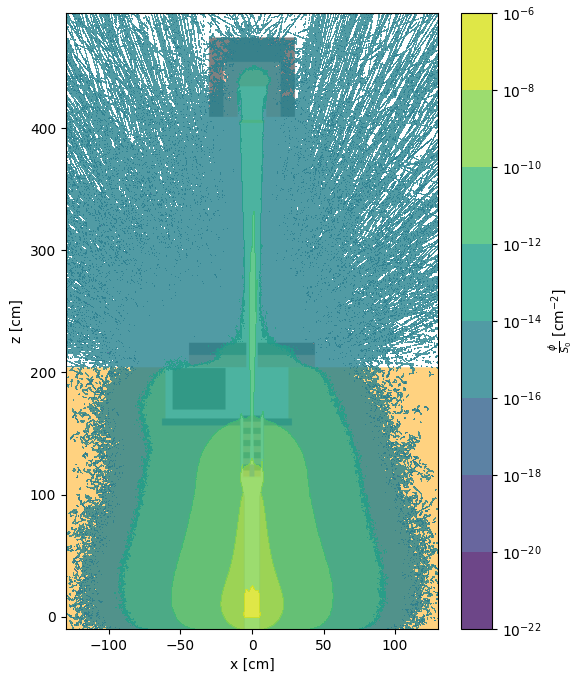
\includegraphics[width=0.7\textwidth]{conducto_flujo.png}
\caption{Distribución del flujo neutrónico en el modelo del conducto Nº5.}
\label{fig:conducto-flujo}
\end{figure}

Este comportamiento justifica la estrategia de desacoplar geométricamente la simulación del conducto respecto del núcleo del reactor. Simular directamente desde el núcleo implicaría combinar la baja probabilidad de que los neutrones alcancen la entrada del conducto con la también baja probabilidad de que atraviesen el colimador y lleguen al banco de detectores, resultando en una estadística reducida. En cambio, al utilizar la fuente distribucional en la entrada del conducto como fuente, se logra concentrar los recursos computacionales en la región de interés, obteniendo una estadística adecuada para el análisis espectral y mejorando los resultados.

\subsection{Comparación con la medición experimental}

La Figura~\ref{fig:conducto-espectro} muestra el espectro neutrónico obtenido en el banco de detectores a partir de la simulación con fuente distribucional, en comparación con el espectro medido experimentalmente mediante TdV. Se observa concordancia a partir de energías del orden de 0.01~eV. No obstante, por debajo de ese umbral, el flujo simulado subestima al medido experimentalmente.

\begin{figure}[h]
\centering
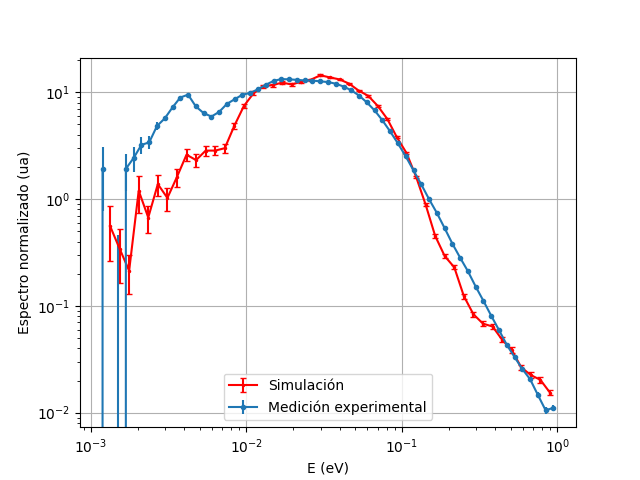
\includegraphics[width=\textwidth]{conducto_espectro.png}
\caption{Comparación del espectro de neutrones obtenido en el banco de detectores en la simulación de \texttt{OpenMC} con la medición experimental realizada por TdV por el Departamento de Neutrones del CAB.}
\label{fig:conducto-espectro}
\end{figure}

Esta discrepancia en la región de bajas energías puede atribuirse principalmente a dos factores:

\begin{itemize}
\item \textbf{Limitaciones en la representación espectral de la fuente}. Tal como se observa en la Figura~\ref{fig:conducto-comparacion-let}, existe diferencia entre el archivo original y la fuente distribucional en la región de mayor letargía, correspondiente a las energías menores a 0.01~eV. Esta desviación se origina en la discretización inherente al método de histogramas.
\item \textbf{Tratamiento del filtro de bismuto en la simulación}. En la modelización realizada con \texttt{OpenMC}, se emplean secciones eficaces correspondientes a átomos de bismuto como gas libre. Sin embargo, el filtro real está construido con bismuto cristalino, cuyas secciones eficaces difieren a bajas energías \cite{Mishra2006PULSTAR}. Mientras que para energías superiores a 0.1~eV ambas secciones eficaces son equivalentes, por debajo de ese valor la sección eficaz del bismuto cristalino es menor. La máxima discrepancia se presenta en torno a 1~meV, donde la sección eficaz del bismuto cristalino representa apenas el 10\% de la correspondiente al bismuto libre. Este efecto conduce a una atenuación del flujo térmico simulado, explicando la subestimación observada en la comparación con los datos experimentales.
\item \textbf{Tratamiento experimental de los datos medidos}. La medición experimental utilizada como referencia ha sido obtenida a partir de mediciones realizadas con detectores de ${}^3$He, y requiere un proceso de postratamiento. Este proceso incluye correcciones por tiempo muerto de los detectores, eficiencia de detección de los detectores de ${}^3$He y por nivel de fondo. En particular, la estimación y substracción del nivel de fondo puede introducir cierta variabilidad en la forma final del espectro, especialmente en la región correspondiente a menores energías. Como es esta la región del espectro donde se registra la mayor discrepancia respecto a la simulación, no puede descartarse que parte del desvío observado esté asociado a incertidumbres propias del procedimiento de corrección experimental aplicado.
\end{itemize}

A pesar de estas limitaciones, los resultados obtenidos permiten validar el enfoque implementado, demostrando que la fuente distribucional construida es capaz de reproducir adecuadamente el comportamiento espectral de los neutrones en el banco de detectores en el rango de interés térmico.
